%%%%%%%%%%%%%%%%%%%%%%%%%%%%%%%%%%%%%%%%%%%%%%%%%%%%%%%%%%%%%%%%%%%%%%%%%%%

\documentclass{standalone}

\usepackage{amsmath}
\usepackage{mathptmx}
\usepackage{pgfplots}
\usetikzlibrary{external}
\tikzexternalize{baseball-x-y-displacement}
\pgfplotsset{compat=1.16}

%% IEEE uses Times Roman font, so we'll default to Times.
%% These three commands make up the entire times.sty package.
\renewcommand{\rmdefault}{ptm}
\renewcommand{\ttdefault}{pcr}
\normalfont\selectfont

\begin{document}

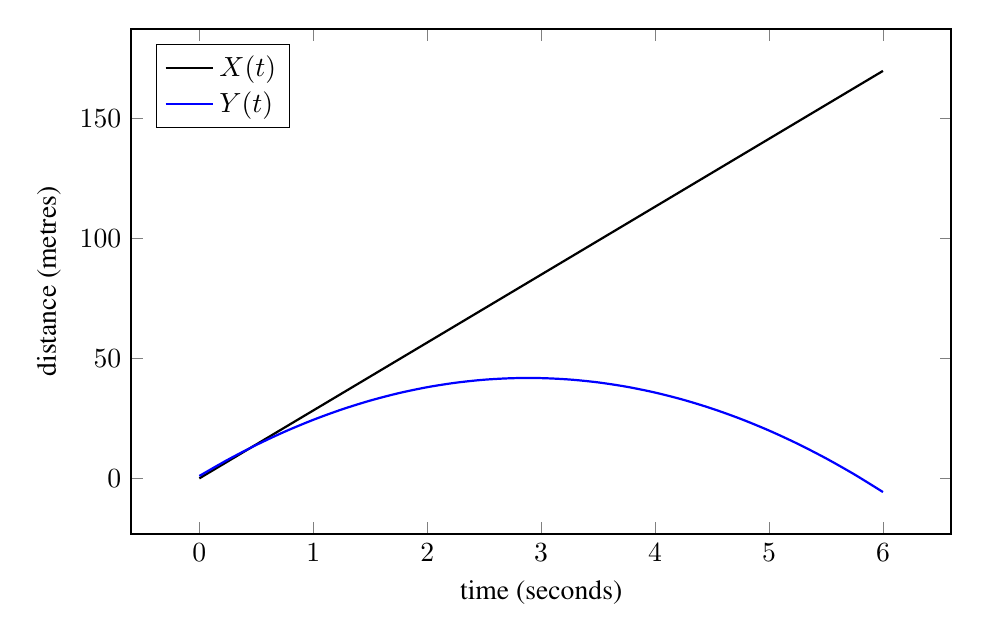
\begin{tikzpicture}
\tikzset{%%
  every mark/.append style={scale=1.0},%%
  scale=1.0%%
}
\pgfplotsset{%%
  every axis/.append style={font=\normalsize}%%
}

\begin{axis}[%%
  axis line style=thick,%%
  enlargelimits=true,%%
  height=8cm,%%
  legend cell align=left,%%
  legend pos=north west,%%
  plotStyle/.style={%%
    domain=0:6,%%
    mark=none,%%
    smooth,%%
    thick%%
  },%%
  width=12cm,%%
  %%
  %% x-axis
  xlabel={\normalsize time~(seconds)},%%
  %%
  %% y-axis
  ylabel={\normalsize distance~(metres)},%%
  ylabel style=above%%
]
%%
%%
%% The horizontal displacement.
\addplot+ [plotStyle,black]
{20 * sqrt(2) * x};
\addlegendentry{$X(t)$}
%%
%%
%% The vertical displacement.
\addplot+ [plotStyle,blue]
{-4.9 * x^2 + 20*sqrt(2)*x + 1};
\addlegendentry{$Y(t)$}
\end{axis}
\end{tikzpicture}

\end{document}
